%&pdflatex
\documentclass{article}

\usepackage{color}
\usepackage{subcaption}
\usepackage{graphicx}
\usepackage{multicol}
\usepackage{geometry}
 \geometry{
 a4paper,
 total={170mm,257mm},
 left=20mm,
 top=20mm,
 }

 \newenvironment{Figure}
  {\par\medskip\noindent\minipage{\linewidth}}
  {\endminipage\par\medskip}



\graphicspath{{./images/}}

\begin{document}
\begin{multicols}{2}

\section{Abstract}     
Paths on the Autonomous Systems (AS) graph of the Internet
derived from the Border Gateway Protocol (BGP) can be used by researchers to
understand the dynamics of Internet topology and to interpret how that
topology may enable nations to enact censorship, surveillance, or other
Internet control measures. Unfortunately datasets of these paths are not
generally made publicly available, and paths collected from measurements such as
traceroute or BGP probes tend to be incomplete. Simulation
frameworks have been used to generate AS paths based on empirical AS graphs.
We have reimplemented and extended one such framework, BGPSim \cite{quicksand} in Python as
an efficient, open source BGP path simulation tool called BGPSimPy. With this
tool we produced publicly available routing tree datasets that will enable
future research on AS level topology. We introduce a metric, \textit{chokepoint potential},
in order to use routing trees to interpret the capability for border ASes (those one hop away from
an AS in a different nation) to enact censorship or surveillance. With the entire set of
routing trees we demonstrate that we can expose the choke points of AS-level routing for
any nation. Previous research endeavors in this
direction have only identified chokepoints in single snapshots. We apply the
path simulation and routing tree datasets to view snapshots of the Internet
over multiple years in order to introduce a new technique to investigate the
evolution of the complex and dynamic AS level Internet topology. Through this approach we
can more carefully evaluate the state of the Internet than was previously possible. As an
application of the routing trees we compare multiple qualitative sources of
Internet freedom and censorship with chokepoint metrics in order to interpret
the relationship between AS level topology and actual censorship activity, providing
illustration of new ways to monitor which governments can easily control the flow of 
information in their nations.

\section{Related Work}
The primary struggle facing Internet topology researchers is
a lack of ground truth data. Paths on the AS level of the Internet are
incomplete and sometimes inaccurate {\color{blue}cite?}. Additionally, AS business
relationships are confidential and not publicly available. In this absence of
solid empirical data, a technique for inferring AS relationships and a
technique for inferring BGP paths are needed to study AS-level topology and
evolution. The first effective relationship inference algorithm was developed
by Gao in \cite{gao}. This algorithm was limited in that it focused on
maximizing the occurrences of the valley-free rule on the AS graph, which has
been shown to not always hold {\color{blue}cite?}. Additionally, Gao's algorithm was
verified against a single tier-1 provider's ground truth data. A more
verifiable correct set of AS relationships was developed by the Center for
Applied Internet Data Analysis (CAIDA) \cite{CAIDApaper}. These relationships,
which were generated using Gao's algorithm and other inference techniques,
were verified against a larger ground truth dataset, and didn't require that
the valley-free rule always hold. This leads to more realistic relationships. AS
relationships do not tell the whole story of AS-level topology, however. In
order to identify chokepoints in the AS graph, it is necessary to determine
the paths that Internet traffic follows. Researchers either use a measurement
tool like traceroute or BGP AS-path announcement data to determine AS paths.
These techniques have been shown to yield an incomplete and innacurate set of
paths {\color{blue}cite?}. 
\par
In light of these issues, BGP researchers often employ more abstract models of BGP.
For instance, the authors in \cite{converge} developed a simplification of BGP in order
to estimate important convergence properties. In order to evaluate Internet chokepoints,
an accurate set of paths between all AS pairs must generated. One technique for generating such
a set of paths was developed by Gill et al. in \cite{quicksand}. The algorithm
developed in \cite{quicksand}, called BGPSim, uses a modified breadth-first
search on an AS graph with defined relationships, as in from the CAIDA
dataset. The breadth first search traverses the AS graph starting from a root
node, and the search traverses edges according to priorities related to the
relationships defined by Gao. The priorities, in the order they are integrated
into the algorithm, are: Shortest Path (SP), Local Preference (LP), and Tie-
break (TB). The resultant paths are ideal according to economic concerns of AS
administrators.     
\par
Previous studies have used BGP path models to find ASes that
intercept a high fraction of paths. One such project in \cite{throats}
identified that 90\% of paths on the Internet could be intercepted with only 30
or so ASes. The researchers in \cite{throats} generated paths by first using
only paths to top websites as defined by the Alexa top websites project,
and then appending additional edges to those paths from the full
AS graph according to the principles defined by Gao \cite{gao}. Many of the
ASes that were found to intercept a large number of paths were found to be
within nations that conduct censorship. As an extension of these results,
another paper \cite{decoy} revealed that ASes that intercept many paths could
be utilized for decoy routing. This approach for identifying AS level
chokepoints has several potential pitfalls that are remedied by the approach
taken in this paper. First, the authors in \cite{throats} didn't consider that
many of the paths found from the Alexa top websites would have destinations in
nations that censor Internet traffic, particularly China due to its large
Internet population. This artificially inflates the chokepoint nature of
Chinese ASes. As an alternative, in this paper we consider paths from every
source-destination AS pair, and we make a distinction between in-to-out paths
and out-to-in paths. Secondly, chokepoints have previously only been
identified at a single snapshot of the Internet. This makes it difficult to
discuss the evolution of Internet topology, and whether or not chokepoints are
anomalous or common. Finally, the aforementioned approach for identifying
chokepoints does not allow a clear comparison between different nations. It
can be said that one nation controls a large portion of Internet paths, but
not how easily traffic directed through that country could be intercepted on a
national level. For this, some aggregate measure across all of the border ASes
within a country must be considered, as it is in this paper.     
\par
In \cite{chinafiltering}, Xu et al. investigated the AS level topology of China
to identify where keyword filtering occurred. They found that the most
effective ASes with which to deploy keyword filtering devices are those in the
backbone of the Chinese AS topology. A relevant contribution of
\cite{chinafiltering} is that, while most filtering occurs in border ASes,
some filtering is controlled by non-central provincial ASes. China has a
diverse strategy for Internet censorship, both targeting chokepoints and the
Chinese provincial network. The potential for various forms of censorship in
regards to various AS level topologies motivates the question: Is centralized
censorship or decentralized censorship more common? Instead of directly
identifying censorship devices on the AS graph, we instead quantify the
chokepoint potential of ASes on the national level, and then compare that with
qualitative Internet freedom measures and empirical censorship events.
\par
We are not the first to investigate the relationship between Internet freedom and
AS-level topology. Similar techniques have been used to classify nations according
to the connectivity of their ASes \cite{politicsrouting}. This has only been done for a
single moment in time, however, making the results limited in terms of stability and predictability.
Additionaly, previous work has not used country level chokepoints as the link between Internet topology
and censorship or surveillance practices. The work in \cite{politicsrouting} chose to relate Internet topology
to the Freedom of the Press measure from freedom house instead of the Freedom On The Net score. They chose to do this
to include more nations. Additionally, they didn't include the United States and Russia in their experiments because they were
outliers in regards to their topologies. Through our approach we hope to extend this previous work by finding an interesting metric for
understanding the dynamics of all nations, as well as targeting our results more specifically to Internet freedom by using the Freedom On
The Net score as our metric for Internet freedom. Through our techniques, we provide a simple metric that not only 
sheds light on the relationship between topology and Internet freedom, but reveals currently free
nations that could easily implement censorship if their governments decided to.

\section{BGPSimPy}
In order to conduct an analysis on AS level topology, the paths
generated by the Border Gateway Protocol (BGP) have to be modeled. A
traditional approach is to use a tool like traceroute to collect paths via
measurement, or at a larger scale use a selection of BGP data collectors with
a tool like BGPStream \cite{bgpstream} \cite{traceroute}. Unfortunately, these
techniques require extensive collection time and are still susceptible to
errors and incomplete data. There is no readily available BGP path dataset
with which to study. Thus, researchers must turn to simulation to find
accurate BGP paths.     
\par One such simulation framework, the previously
mentioned BGPSim, was developed by Gill et al. \cite{quicksand} as a tool for
quickly estimating AS paths from an input AS graph. This AS graph could be
taken from a set of inferred AS relationships, such as the CAIDA AS
relationship dataset \cite{CAIDA}. BGPSim outputs routing trees, which contain
all paths from leaf ASes to the root AS, for each AS in the AS graph. The
routes are selected using a modified breadth-first search that selects with
the following priorities: shortest path, local preference (using the rules
from Gao \cite{gao}), and finally tie break of all equally good paths. With
these priorities, BGPSim generates a realistic collection of AS level paths,
which are ideal for use in Internet topology studies.
\par 
Unfortunately, BGPSim is not ready to deploy immediately and easily, as would be necessary
for a tool dedicated to allow fast monitoring of the Internet's overall state.
This is largely due to the fact that BGPSim is written in C\# (affecting its
ability to be used in a cross-platform way) with DryadLinq (a deprecated C\#
library) for distributed computing. As a remedy to these problems, we have
reimplemented BGPSim under the name BGPSimPy. BGPSimPy is written purely in
python, making it cross platform and easy to integrate. Additionally,
distributed computing is now achieved with MPI using mpi4py, a framework that
is supported on many computer clusters.

\section{Generating Routing Trees}
AS level Internet topology research is plagued
by a lack of publicly available path data. Path inference is also
computationally expensive for the entire Internet, prohibiting continuous
research and Internet monitoring. Thus, we have chosen to release the routing
tree datasets generated for this paper. This is a major contribution to
Internet research, and will allow new endeavors to investigate Internet
topology relationships on an unprecedented scale. As a focus of this paper,
and an example application, we use these routing trees to examine topological
evolution of the Internet and its relationships to Internet freedom and
censorship.

\section{Applications of Routing Trees}
\subsection{Measuring Chokepoints in AS-level Paths}

It is well documented that the AS graph is composed of a hierarchy of ASes, such that the ASes
distributed in tiers. This tier list includes a very small set of tier-1 ASes
that are able to provide the highest levels of connectivity to the rest of the Internet \cite{hierarchy}.
This hierarchy is generally viewed in a way agnostic to national boundaries. It is
possible, however, that more ASes exhibit potential to control information flow in the sense that
chokepoints can exist at the national level. While these chokepoints might not provide extensive connectivity
to the entire set of ASes, they may provide similar connectivity to the interior ASes of a particular nation. 
Thus, a technique to conduct a fine-grained analysis of the number of paths intercepted by ASes that provide access
in and out of nations is a worthwhile pursuit. Previous works have also not provided an analysis of the development of
the AS hierarchy over time. The monitoring of national chokepoints over time is relevant to predicting the stability of the
future Internet, identifying key censorship bottlenecks, and understanding the potential for national governments to conduct
surveillance on foreign traffic.

\par

Once we generated routing trees using BGPSimPy, we
used the paths to identify national chokepoints. Specifically, we chose to evaluate border
ASes, or ASes that could reach an AS registered to a different nation with one
hop. By selecting border ASes we could locate the ASes that intercepted
traffic into a nation (via out-to-in paths), as in a foreign attempt to access
a domestic website, or ASes that intercepted traffic out of a nation, as in a
domestic attempt to access a foreign website (via in-to-out paths). We choose
to make a distinction between these two path types to better understand the
implications of the chokepoints belonging to each nation.

\par To evaluate border ASes we use the metric of chokepont potential, defined here to be the
ratio of the number of paths intercepted by a border AS to the number of total path interceptions
possible for that nation. If $P_c$ is the set of all paths (either in-to-out or out-to-in) belonging to nation $c$ and 
$B_p$ is the set of all border nodes within a path $p$, the chokepoint potential for a border node $b$ is defined in equation \ref{eqn:chokePointPotential}
This metric is calculated separately for both in-to-out paths and out-to-in paths.
This calculation is performed by traversing the routing trees and keeping
record of which border nodes intercept each path, as well as what path type is
currently being traversed with regards to the host nation of the border AS in
question. Once all paths are traversed, the totals are compiled together, with
a chokepoint potential value stored for each border AS.

\begin{equation}\label{eqn:chokePointPotential}
CP_b = \frac{|\{p \in P_c \textrm{ s.t. } \{b\} \subseteq B_p\}|}{\sum_{p \in P_c}|B_p|}
\end{equation}

\par 
The chokepoint potentials of the border ASes allowed us to investigate the state of the AS-
level topology of the Internet for any given set of initial AS relationships.
We first looked at how many ASes each nation is required to control to
intercept a percentage of paths. For this test, we chose 90\%, as this would
indicate a clear control of Internet paths for the given country and was also
the percentage used in past studies \cite{throats}. Additionally, we determined this value
for each nation for multiple timestamps, yielding our initial picture of the
evolution of Internet topology. The results of this test for some nations of
interest are shown in figure \ref{fig:NumToIntercept}.

\begin{Figure}
	\centering
	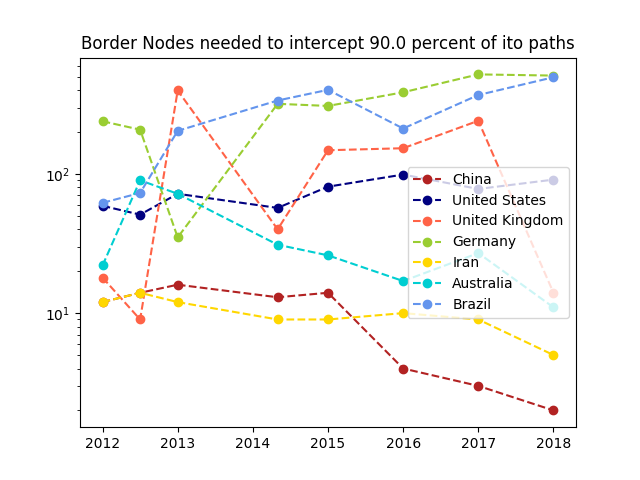
\includegraphics[width=\linewidth]{NodesNeeded}
	\captionof{figure}{Number of border nodes needed to control 90\% of paths for various nations}\label{fig:NumToIntercept}
\end{Figure}

\par
These results give an idea of how the Internet has evolved for different nations. Some nations,
particularly China, have evolved to a state where it is significantly easier
to intercept paths. Others, for instance Brazil, have become more open with
regards to the chokepoint nature of border ASes. These results are even more
striking when one considers that the number of ASes globally has drastically
increased over the years, amplifying the effect of higher chokepoint
potentials. The number of ASes in the CAIDA AS relationship dataset in 2012
was 43,274 in January, while in January of 2018 the count was 60,006.
Next, we took a more fine-grained approach to investigate the dynamics and
evolution of AS-level chokepoints. For each nation, we sorted the border ASes
in descending order into a list, so that the first AS in the list was the AS
with the highest chokepoint potential. Then, we selected each AS from the list
and kept track of the ratio of paths intercepted. This test allowed us to
investigate the ease with which different nations could control paths at
multiple timestamps. Additionally, this experiment illuminates that the
topological state of a nation in regards to border ASes is often complex and
dynamic. Since nations possess wide variations in AS count, this data is best
visualized on a semi-logarithmic scale. The different timestamps are shown in
different colors, where red is the furthest in the past and blue is the most
recent. These results are depicted in \ref{fig:chokepoint}. 

\begin{figure*}
	\centering
	\begin{subfigure}[b]{0.4\linewidth}
		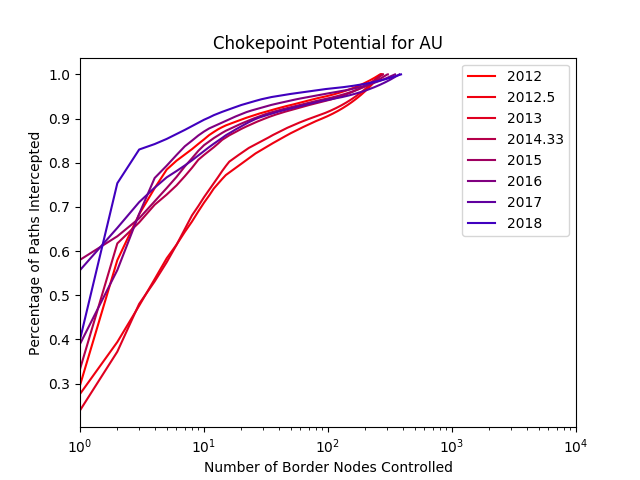
\includegraphics[width=\linewidth]{single_AU}
	\end{subfigure}
	\begin{subfigure}[b]{0.4\linewidth}
		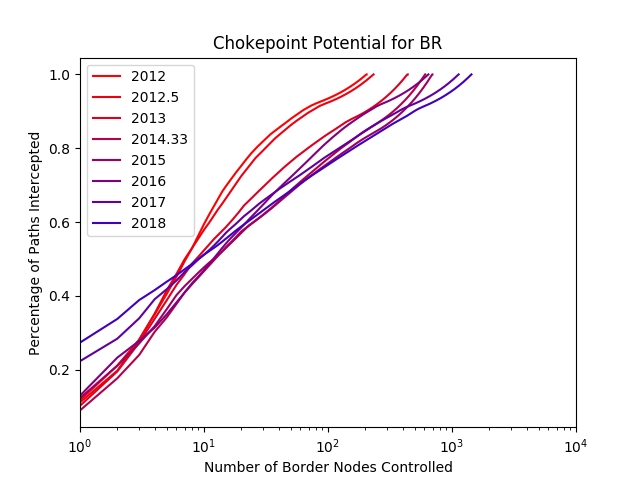
\includegraphics[width=\linewidth]{single_BR}
	\end{subfigure}
	\\
	\begin{subfigure}[b]{0.4\linewidth}
		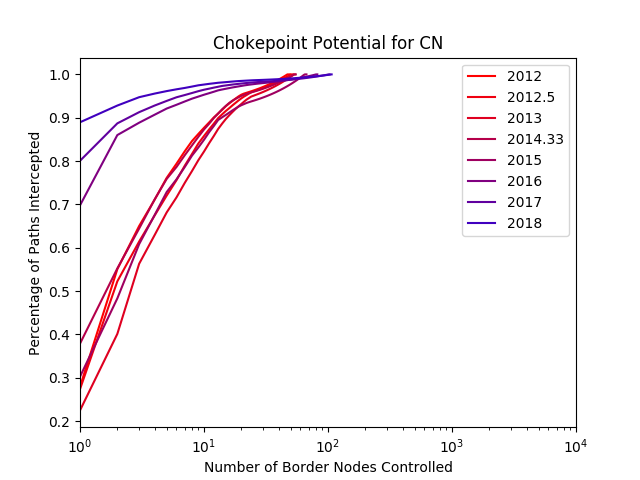
\includegraphics[width=\linewidth]{single_CN}
	\end{subfigure}
	\begin{subfigure}[b]{0.4\linewidth}
		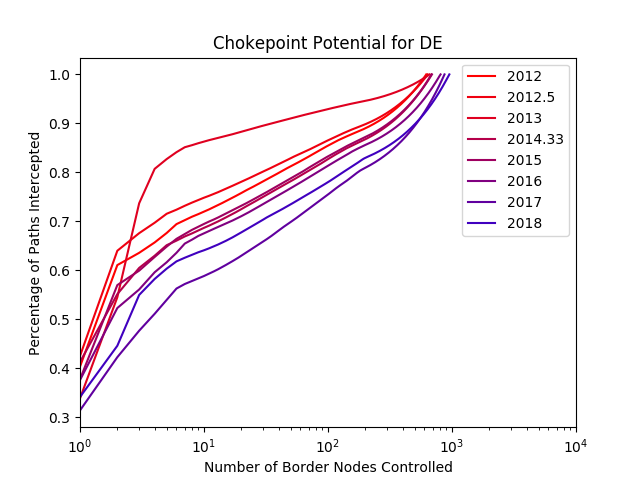
\includegraphics[width=\linewidth]{single_DE}
	\end{subfigure}
	\\
	\begin{subfigure}[b]{0.4\linewidth}
		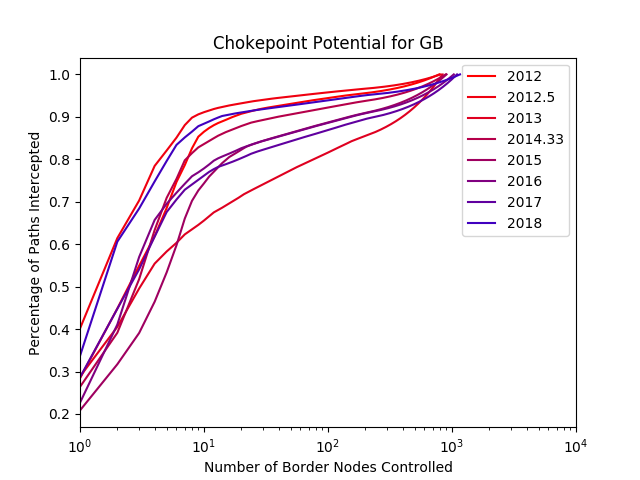
\includegraphics[width=\linewidth]{single_GB}
	\end{subfigure}
	\begin{subfigure}[b]{0.4\linewidth}
		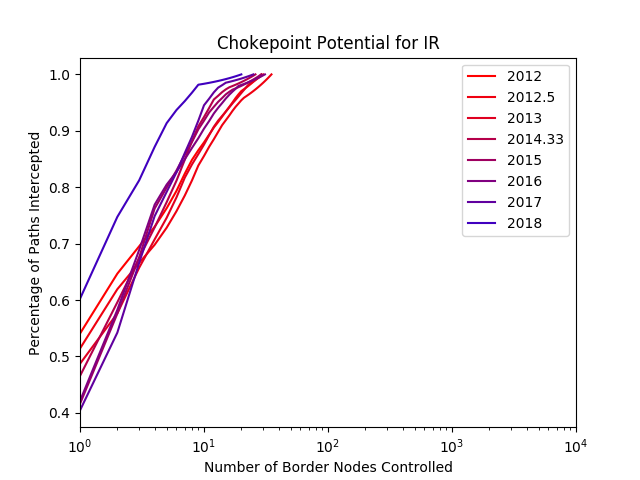
\includegraphics[width=\linewidth]{single_IR}
	\end{subfigure}
	\\
	\begin{subfigure}[b]{0.4\linewidth}
		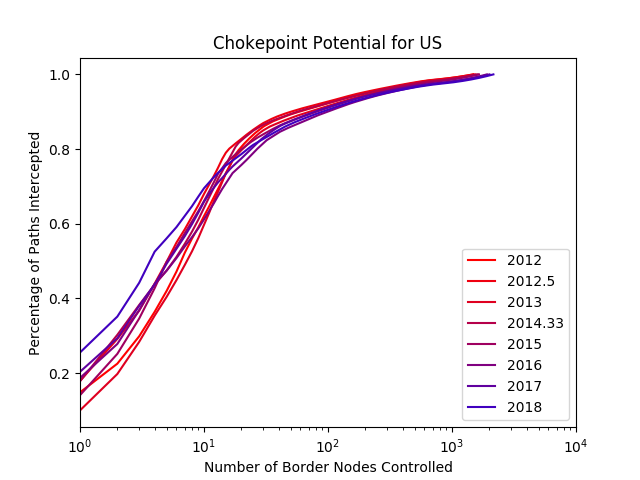
\includegraphics[width=\linewidth]{single_US}
	\end{subfigure}


	\caption{Ratio of Paths Intercepted for a certain number of Border Nodes for multiple nations}\label{fig:chokepoint}
\end{figure*}

\par 
The variation between the different nations highlights the importance of measuring
chokepoints on the national level. Trends exist within a nation, but nations
tend to have surprisingly unique AS graph dynamics. China shows a striking
increase in chokepoint potential. In order to control 90\% of paths, China has
to utilize a strikingly few number of ASes. This suggests an ever
strengthening backbone in the Chinese Internet. Conversely, the trend that
Brazil's capability to intercept paths is decreasing is also evident in these
results. This could be the effect of an expansion of infrastructure, leading
to more border ASes and more diverse paths in and out of the country. {\color{blue}Maybe
there is a source to support this?} Another interesting element of these
results is the dynamic behavior for some nations. It seems that in some cases,
when it becomes easier to control many paths, it becomes more difficult to
control all paths. {\color{blue}Not sure of implications, needs work here}

\subsection{Comparing Internet Topology with Freedom On The Net}
While research in the past has connected AS-level topology with Internet freedom 
and censorship \cite{throats}\cite{politicsrouting}, the evolution of this relationship has
not been investigated across multiple years. We also provide the first attempt to connect the
metric of chokepoint potential with the Internet freedom of nations, creating insight into the
connection between the state of Internet topology and efforts to limit Internet freedoms.
\par Freedom House's Freedom On The Net
(FOTN) report \cite{FOTN}, is an annual ranking and analysis of Internet
freedom, interpreted from multiple measures including obstacles to access,
limits on content, and violations of user rights. The FOTN includes a ranking
of nations by a freedom index, where a higher number indicates a less free
Internet for that nation. The index is calculated from a series of questions
that are evaluated according to various sources regarding each nation. These
questions encompass multiple categories, including government filtering and
censorship of web traffic. In order to investigate whether the topology of a
nations ASes is related to Internet freedom, we compare the FOTN freedom index
with the ease with which a nation can control AS level paths. In figure
\ref{fig:fotn} we plot the number of ASes required for a nation to control 90%
of paths with that nation's freedom index for multiple timestamps of AS
relationships.

\begin{figure*}
	\centering
	\begin{subfigure}[b]{0.4\linewidth}
		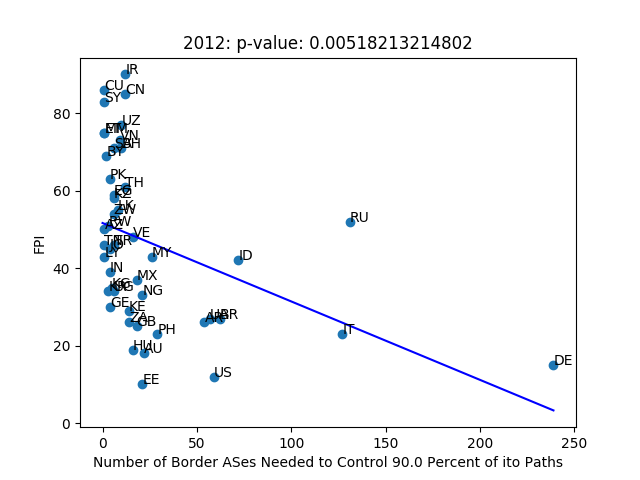
\includegraphics[width=\linewidth]{fotn2012}
	\end{subfigure}
	\begin{subfigure}[b]{0.4\linewidth}
		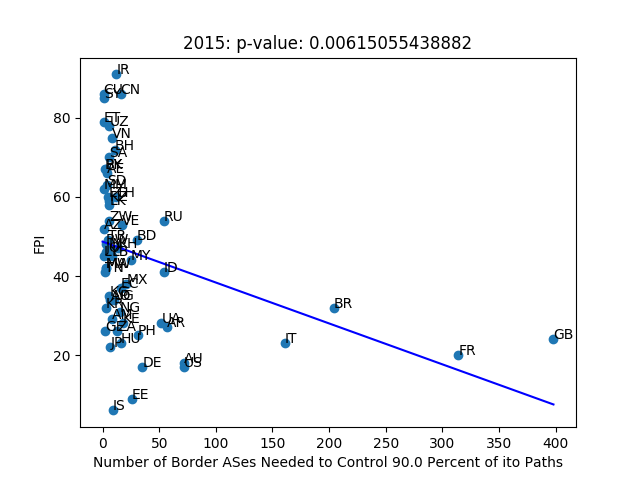
\includegraphics[width=\linewidth]{fotn2015}
	\end{subfigure}
	\\
	\begin{subfigure}[b]{0.4\linewidth}
		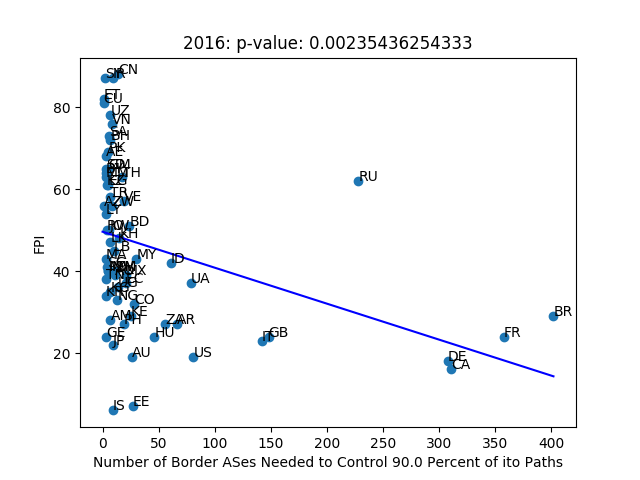
\includegraphics[width=\linewidth]{fotn2016}
	\end{subfigure}
	\begin{subfigure}[b]{0.4\linewidth}
		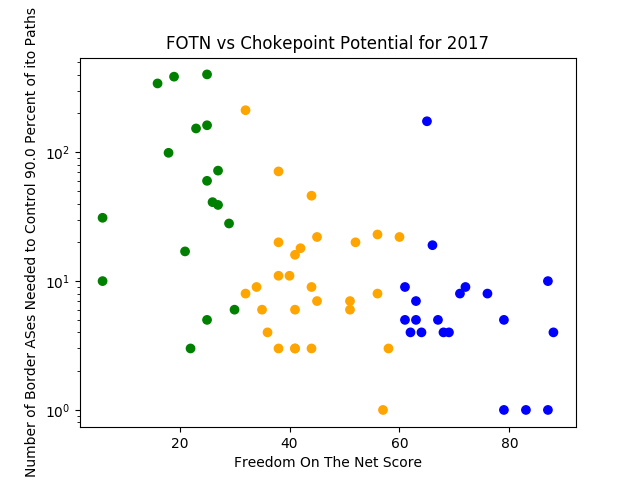
\includegraphics[width=\linewidth]{fotn2017}
	\end{subfigure}


	\caption{Ratio of Paths Intercepted for a certain number of Border Nodes for multiple nations}\label{fig:fotn}
\end{figure*}

\par For each date we fit the data with an ordinary least
squares linear regression, and found the relationship to be statistically
significant (all p-values are less than 0.05). {\color{blue}need some better way to show
exact p-values} The relationship shows that more free nations, as determined
by FOTN scores, tend to have a more difficult to control AS-level topology, as
in border nodes that control fewer portions of paths in and out of that
country. This suggests that either the desire of national governments to
control Internet traffic has impacted the layout of AS relationships, the
topology of the modern Internet has evolved in a way to enable more successful
filtering and blocking, or a combination of both. Up to this point it has been
assumed that Internet topology and Internet censorship are related, but this
has not been supported by both a measure of Internet freedom and actual AS-
level paths.

\subsection{Comparing Internet Topology with Empirical Censorship Data}

Another
technique for relating our chokepoint metric with censorship is to look at
empirical censorship data. One such dataset is provided by the Open
Observatory of Network Interference (OONI) \cite{OONI}. OONI is a project
wherein Internet users around the world use a tool (the ooniprobe) to examine
evidence of Internet censorship. The ooniprobe allows users to run a series of
tests, such as an HTTP requests that might be known to be blocked by certain
nations. The ooniprobe then compares the results of tests with previously
determined unblocked examples of the same tests. Results where the test
differs from expected are considered anomalies, and further heuristics can
determine if the anomalies are likely to be censorship events.
\par We examined
18 days of OONI data from January in 2018. We recorded the ratio of anomalies
in measurements for several classes of anomalous behavior to total
measurements carried out in each nation. We used the web connectivity test
from OONI that records the following fields to measure connectivity: DNS,
HTTP\_FAIL, HTTP\_DIFF, and TCP. Each of these fields are recorded as true or
false, according to whether the test resulted in a potential censorship event.
We then plotted the ratio of potential censorship events in the dataset
against a national metric of chokepoint potential. In this case, we again
looked at the number of border nodes required to intercept 90\% of AS-level
paths. The results of this test are plotted in figure \ref{fig:ooni}. A
relationship like the one seen in the FOTN data is not as clear, perhaps due
to the uneven sampling across nations. It is clear, however, that nations can
be classified both by its chokepoint potential and the occurrence of possible
censorship events. A nation, for instance, with a high ratio of web
connectivity anomalies with a high chokepoint potential can be considered a
censorship active nation with a strongly hierarchical AS topology. Thus, this
analysis serves as a monitoring tool for the state of nations on the Internet
in regards to actual censorship implementation, and potential for further
censorship.

\begin{figure*}
	\centering
	\begin{subfigure}[b]{0.4\linewidth}
		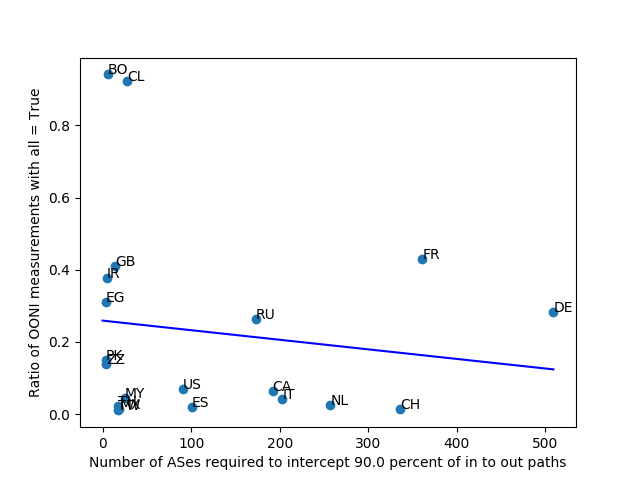
\includegraphics[width=\linewidth]{all_09}
	\end{subfigure}
	\begin{subfigure}[b]{0.4\linewidth}
		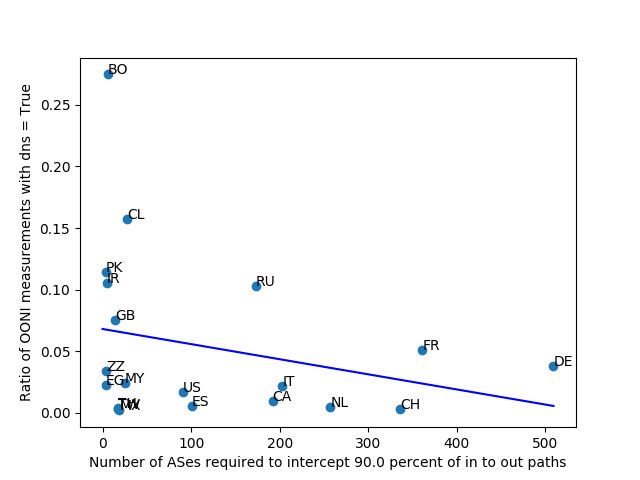
\includegraphics[width=\linewidth]{dns_09}
	\end{subfigure}
	\\
	\begin{subfigure}[b]{0.4\linewidth}
		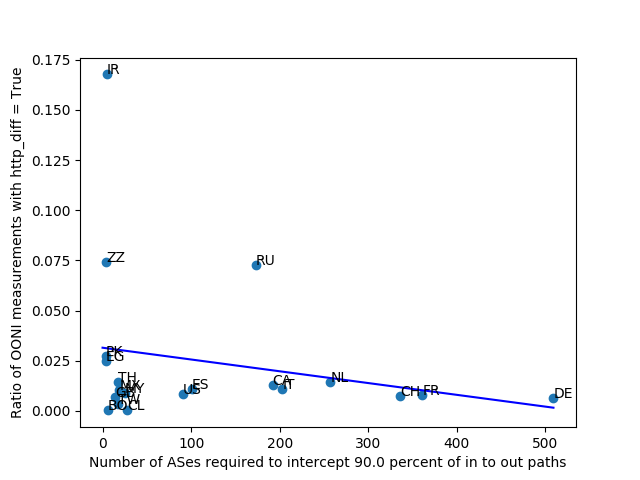
\includegraphics[width=\linewidth]{http_diff_09}
	\end{subfigure}
	\begin{subfigure}[b]{0.4\linewidth}
		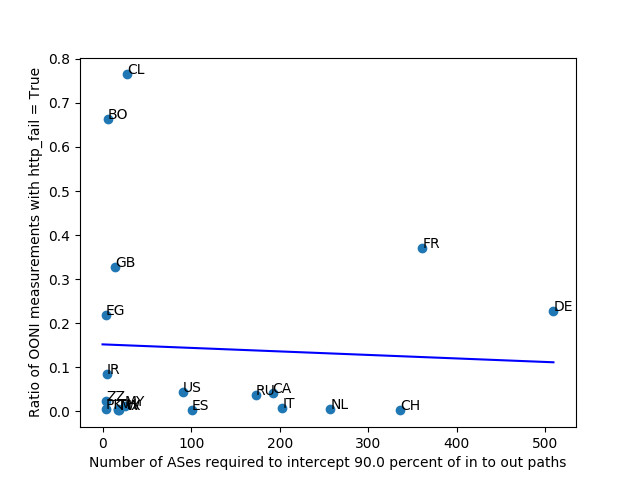
\includegraphics[width=\linewidth]{http_fail_09}
	\end{subfigure}
	\\
	\begin{subfigure}[b]{0.4\linewidth}
		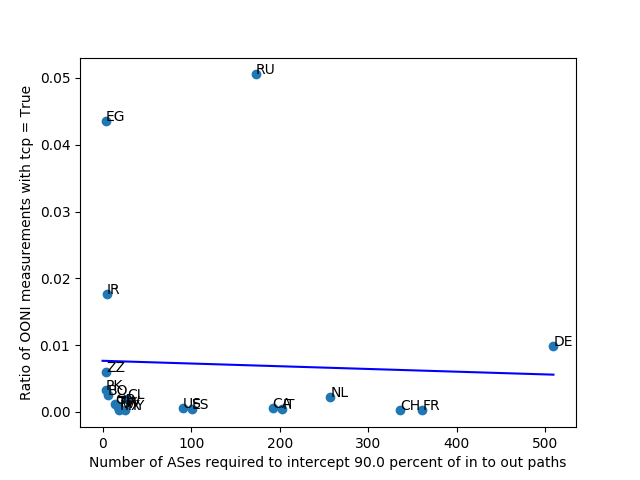
\includegraphics[width=\linewidth]{tcp_09}
	\end{subfigure}


	\caption{Ratio of anomalies in OONI measurements compared to chokepoint potential}\label{fig:ooni}
\end{figure*}

\section{Discussion}

We have introduced an efficient technique for studying the AS-level topology of the Internet. Additionally,
we introduced the metric of chokepoint potential in order to evaluate the control that border nodes possess
over paths into and out of a nation. We have applied the routing trees generated by BGPSimPy along with the
chokepoint potential metric to present an overview of the evolution of the amount and strength of chokepoints
on the AS graph over the past 6 years. We also connected our analysis of AS-level chokepoints in a novel way to
both qualitative measures of Internet freedom and empirical censorship data. The former comparison reveals
a strong relationship between the chokepoint potential of a nation and its lack of Internet freedom, while the
former provides insight into the categories of nations, in regards to their implementations of censorship and
the layout of their AS relationships.

\end{multicols}

\bibliographystyle{plain}
\bibliography{paper}

\end{document}\grid
